\section{Theorie}
\label{sec:Theorie}

Ein Geiger-Müller Zählrohr wird dazu verwendet inonisierende Strahlung auf Eigenschaften wie die Intensität oder Energie zu untersuchen.
Im wesentlichen besteht er aus einem Hohlzylinder aus Metall, welcher die Kathode ist und einem Draht in der Mitte des Zylinders, welcher die Anode ist. (Siehe \autoref{fig:aufbau})
Somit wird im Hohlzylinder bei angelegter Spannung $U$ ein radialsymmetrisches elektrisches Feld erzeugt.
Gefüllt ist das Rohr mit einem Gasgemisch, welches meistens aus überwiegend Argon mit etwas Alkohol besteht.
Geschlossen wird das Zählrohr meistens mit einer sogenannten Mylar-Folie, also Polyester Folie, welche auch $\alpha$-Strahlung durchlässt.
Außerdem wird das Rohr mit einem Spannungsmesser/Stromzähler verbunden.

\begin{figure}
    \centering
    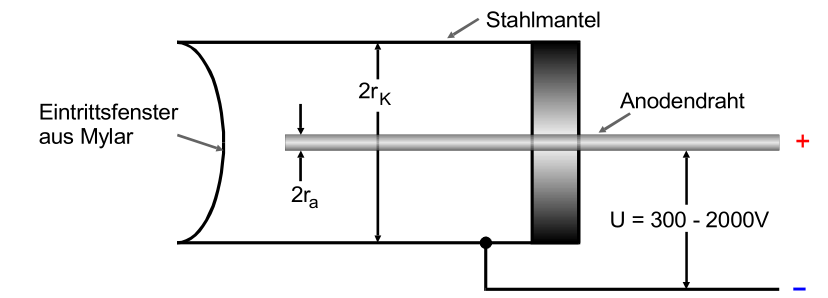
\includegraphics[width=0.9\textwidth]{images/skizze_0.png}
    \caption{Aufbau eines Geiger-Müller Zählrohrs\cite{V703}}
    \label{fig:aufbau}
\end{figure}

\subsection{Spannungsabhängigkeit des Zählrohrs}
\label{ssec:wirkungsweise}

Betrachte werden ionisierende Teilchen, also Teilchen, welche genug Energie besitzen um von bestimmten Atomen ein Elektron zu lösen und somit ein Teilchenpaar mit positiver und negativer Ladung erzeugen.
Die Energie um beispielsweise ein Argon Atom zu ionisieren liegt bei etwa $\SI{26}{\electronvolt}$ wobei die typische Teilchenenergie der betrachteten Strahlung bei über $\SI{100}{\kilo\electronvolt}$ liegt.
Wenn also ein einfallendes Teilchen auf ein Argon Atom trifft, wird ein Ionenpaar erzeugt, das Teilchen verliert einen Teil seiner Energie und fliegt weiter im Gasgemisch.
Es wird also solange Ionenpaare erzeugen, solange es noch genug Energie besitzt.

Durch das elektrische Feld werden so erzeugte positive Ionen zum Zylindermantel beschleunigt.
Entsprechend werden die erzeugten Elektronen zum Anodendraht beschleunigt und erzeugen hier einen Ionisationsstrom zur Kathode.
Wie nun aus diesen Ionenpaaren eine Messung geschehen kann hängt stark von der angelegten Spannung ab und kann grob in vier Spannungsbereiche unterteilt werden. (Siehe \autoref{fig:spannung})

\begin{figure}
    \centering
    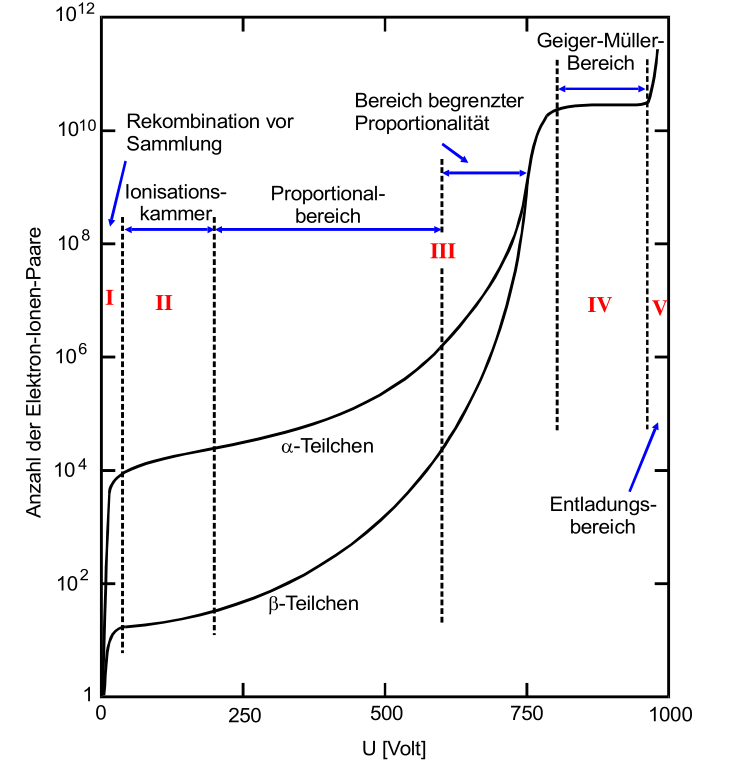
\includegraphics[width=0.7\textwidth]{images/skizze_1.png}
    \caption{Wirkungsweise des Zählrohrs in Abhängigkeit der angelegten Spannung}
    \label{fig:spannung}
\end{figure}


Im ersten Bereich, also bei sehr niedriger angelegter Spannung ist die Beschleunigung nicht groß genug um die Ladungen dauerhaft zu trennen.
Hier führen Rekombinationsprozesse dazu, dass nur einige der Ionen die Annode oder Kathode erreichen.
Den Zähler in diesem Spannungsbereich zu verwenden ist also wenig sinnvoll.

Erhöht man die Spannung werden immer weniger Ionenpaare aufgrund von Rekombination neutralisiert.
Und man kann nahezu alle erzeugten Ladungen an der Anode/Kathode erwarten.
Somit ist der Ionisationsstrom abhängig von der Energie und Intensität der einfallenden Strahlung.
Dieser Spannungsbereich wird für sogenannte Ionisationskammern verwendet.

Bei noch höherer Spannung (Bereich 3 in \autoref{fig:spannung}) werden mehr Ionenpaare erzeugt, als die Energie des einfallenen Teilchens erzeugen kann.
Dies geschieht dadurch, dass die erzeugten Elektronen im elektrischen Feld nahe der Anode so beschleunigt werden, dass diese ebenfalls ionisierend werden und somit weitere Ionenpaar erzeugen, welche wiederum ionisierend wirken können.
Dieser lawinenartige Vorgang wird auch Townsend-Lawine genannt.
Allerdings ist die Anzahl der erzeugten Ionenpaare trotzdem abhängig von der Energie der einfallenden Strahlung.
Hier spricht man von einem Proportionalzählrohr.

Ab einer bestimmten Spannung ist die Anzahl der erzeugten Ionenpaare nicht mehr Abhängig von der Energie der einfallenden Strahlung.
Dieser Bereich (Bereich 4 in \autoref{fig:spannung}) wird als Auslösebereich bezeichnet und ist der Bereich, in dem man von einem Geiger-Müller Zählrohr spricht.
Hier werden die erzeugten Elektronen so stark beschleunigt, dass sie beim Stoß mit einem Argon Atom zusätzlich ionisierende Photonen erzeugen können, welche senkrecht zum elektrischen Feld fliegen können.
Somit werden durch den Ionisationsprozess des einfallenden Teilchens über das ganze Zählrohr Ionenpaare erzeugt und die Anzahl ist nicht mehr abhängig von der Energie der einfallenden Strahlung.
Hier kann nur noch die Intensität der einfallenden Strahlung gemessen werden, also wie viele Teilchen pro Zeit ins Zährrohr absorbiert werden.

Im letzten Spannungsbereich führt ein Ionisierungsprozess zu dauerhaften Nachentladungen und das Zählrohr ist praktisch nutzlos.

\subsection{Einige Kenndaten des Zählrohrs}
\label{ssec:totzeit}

Aufgrund ihrer höheren Masse werden die positiven Ionen im elektrischen Feld deutlich langsamer beschleunigt als die Elektronen.
Somit kommt es nach einer gewissen Zeit zu einem Überschuss positiver Ladungen im Zylinder und das elektrische Feld in Drahtnähe wird so abgeschwächt, dass nur noch wenige Townsend-Lawinen ausgelöst werden können.
Also kann in einem gewissen Zeitabschnitt nach Messung eines einfallenden Teilchens kein weiteres Teilchen gemessen werden.
Dieser Zeitabschnitt wird Totzeit genannt.

In der Erholungszeit danach werden Ionen welche auf die Kathode treffen mit Elektronen rekombiniert und somit neutralisiert.
Somit entsteht nach der Erholungszeit wieder ein neutral geladenes Gasgemisch im Zählrohr.
Diese Zeit kann allerdings dadurch unterbrochen werden, dass der Rekombinationsprozess Photonen aussendet welche wiederum eine Townsend-Lawine auslösen können.
Dies sind dann Nachentladungen und imitieren somit fälschlicherweise einen Prozess, der als einfallendes Teilchen gedeutet werden kann.
Um die Nachentladungen so gering wie möglich zu halten wird dem Argongas ein Alkoholgas untergemischt.
Auf dem Weg zur Kathode stoßen die positiven Ionen dann mit den Alkoholmolekülen zusammen und geben einen Großteil ihrer Energie ab.
Diese werden zwar ionisiert, aber der Rekombinationsprozess kann aufgrund einer niedrigeren Ionisierungsenergie keine Townsend-Lawine mehr auslösen, sondern es werden Schwingungen ausgelöst.

Der Arbeitsbereich des Geiger-Müller Zählrohrs ist der nahezu konstante Bereich 4 in \autoref{fig:spannung} und wird auch Plateau genannt. 
Da allerdings kein Zählrohr perfekt arbeitet, steigt das Plateau an. Je geringer der Anstieg ist, desto qualitative hochwertiger wird das Zählrohr eingeschätzt.

Das sogenannte Ansprechvermögen des Zählrohrs beschreibt wie häufig ein Teilchen zwar in das Zählrohr einfällt aber nicht detektiert wird.
Je geringer die Energie der Strahlung, desto geringer ist das Ansprechvermögen.